%%\normalsize

%%	Resumidamente: se uma Escola primaria tem turmas do 1\textordmasculine\space ao 5\textordmasculine\space ano, são 8 meses letivos por ano, 4 semanas por mês, se levarmos os alunos 1 vez por semana ao Laboratório de Informática, entao são 5 x 8 x 4 = 160 atividades didaticas, que precisam ser defindas por escrito, apenas uma vez.

\ThisCenterWallPaper{1}{./IMG-GIT/marvin.jpg}

\Large

\begin{itemize}
	\item Professor
	\item Coordenador
	\item Diretor
	\item Secretario de Educação
	\item Supervisor
\end{itemize}

\vfill
\pagebreak

\ThisCenterWallPaper{1}{./IMG-GIT/marvin.jpg}


		
%		\begin{itemize}
%			\LARGE 	\item 1\textordmasculine\space dia de aula
%			\Large	\item 1\textordfeminine\space ano
%			\item 1\textordfeminine\space aula no Lab de Informática
%			\item 1\textordfeminine\space contato com o computador!
%			\LARGE	\item Qual atividade?
%		\end{itemize}
	
	{	\LARGE
		
		\begin{itemize}
			\item Laboratório de Informática
			\Large\item  Próxima 2\textordfeminine\space feira: 
		\subitem 3\textordmasculine\space ano B apocalíptico
			\subitem Qual atividade EXATAMENTE?
		\subsubitem Programa?
		\subsubitem Imagens?
		\subsubitem Arquivos?
		\subsubitem Projetor?
		\subsubitem Equipamentos e materiais adicionais?
		\subsubitem Links?
		\end{itemize}


\vfill
\pagebreak

	
\begin{multicols}{2}
\begin{itemize}
	\LARGE
	 	\item {\LARGE Escola primária}
	\item 1\textordmasculine\space$\rightarrow$ 5\textordmasculine\space anos
	\item ate 400 alunos
	\item 21 máquinas == 20 alunos / aula
    \item 1 aula / turma $\ast$ semana 	\item 8 meses letivos por ano
    \item 4 semanas / mês
    \item 4 turmas / dia
    \item 8 $\ast$ 4 == 32 aulas / ano $\ast$ turma
    \item 20 turmas / semana
    \item 20 turmas * 32 semanas == 
    \item  {\LARGE \textbf{640} atividades}
    
    \vfill\null
    \columnbreak
    \item {\LARGE Por escrito!}
    		\begin{itemize}
    	{\Large  	
    		\item Quem
    		\item Como
    		\item Quando
    		\item Onde
    	\item O quê
    	}
    \end{itemize}
\end{itemize}   

\begin{center}
	\begin{center}
		
\includegraphics[width=\linewidth]{./IMG-GIT/cristal.jpg}
	\end{center}
\end{center}

\end{multicols}   

\vfill\null
\pagebreak

\begin{center}
	
\includegraphics[height=.7\textheight]{./IMG-GIT/anjo.jpg}
	
		\resizebox{\linewidth}{20mm}{\color{magenta}\textbf{Não tem aula de Informática!}}
\end{center}

   \vfill
\pagebreak

%\begin{center}
%	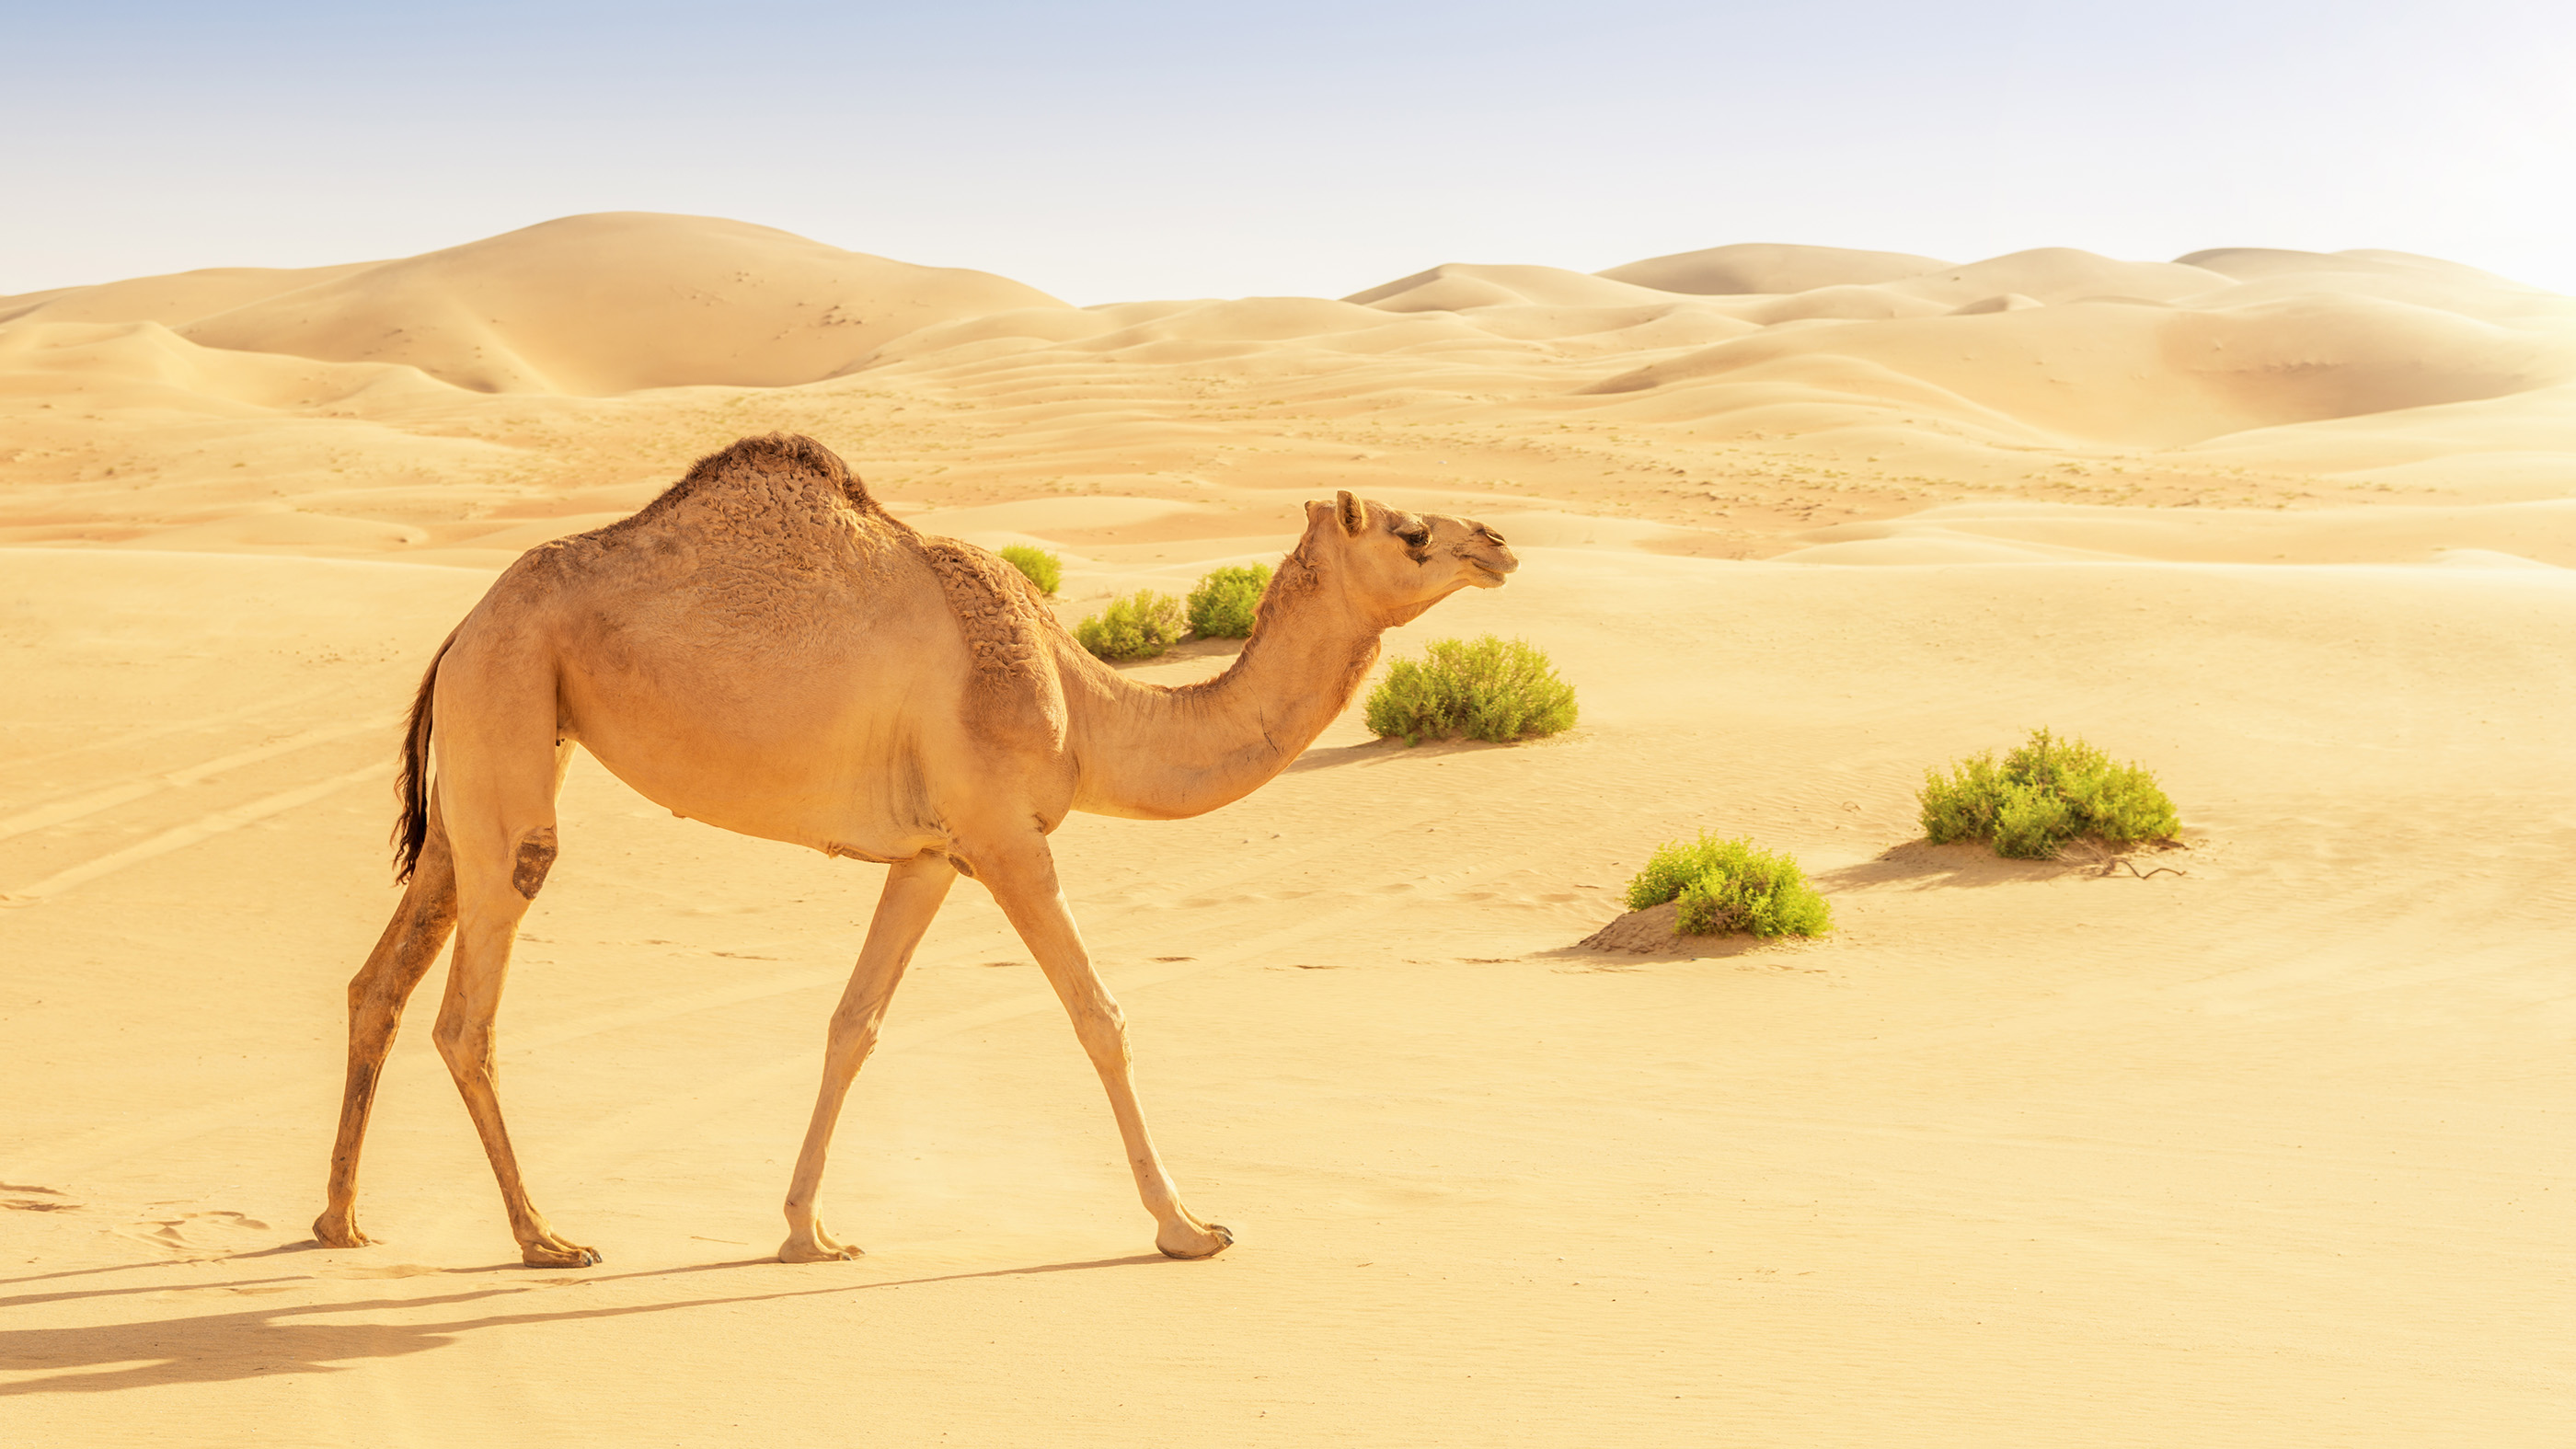
\includegraphics[height=.9\textheight]{./IMG-GIT/camel.jpg}
%\end{center}
%
%   \vfill
%\pagebreak



	\begin{itemize}
		\item  {\LARGE 640 atividades}	
		\item  640 atividades $\ast$ 20 alunos == \textbf{12.800 atividades individuais}.
		\item \textbf{5 linhas de código Shell}
		\item 5 $\ast$ 12.800 == \textbf{64.000} linhas/ano
		\item \textbf{400} linhas/dia
		\item Por escrito.
		\item Em código Shell.
		\item if (hora \textbf{$\geq$ 7:50} da manhã)	
	\end{itemize}

   \vfill
\pagebreak

\vspace*{15mm}
\begin{center}
			\resizebox{.5\linewidth}{.5\textheight}{\color{black}\textbf{8:00}}
\end{center}
		
		   \vfill
		\pagebreak

\ThisCenterWallPaper{1.2}{./IMG-GIT/enchente.jpg}
\begin{center}
	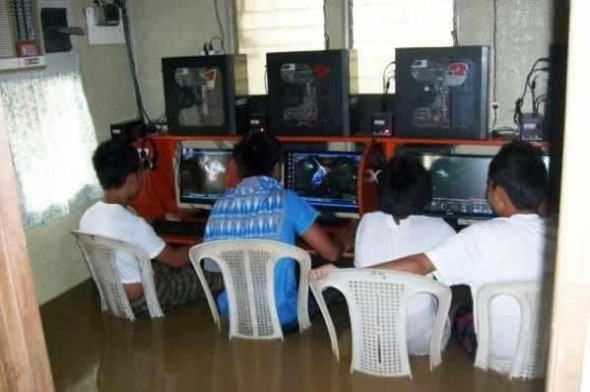
\includegraphics[height=.9\textheight]{./IMG-GIT/enchente.jpg}
\end{center}


\vfill
\pagebreak

\begin{center}
	
\includegraphics[height=.7\textheight]{./IMG-GIT/anjo.jpg}
	
	\resizebox{\linewidth}{20mm}{\color{magenta}\textbf{Não tem aula de Informática!}}
\end{center}

\vfill
\pagebreak


\begin{multicols}{2}
	
	\begin{center}
		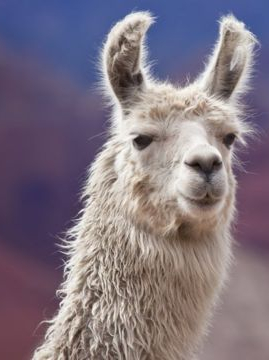
\includegraphics[height=\textheight]{./IMG-GIT/lhama.jpg}
		
		\resizebox{\linewidth}{15mm}{\color{black}\textbf{Lhamento!}}
	\end{center}		
	
	\begin{itemize}
		
		\large
		\item Servico Público.
		\item Jurisprudência.
		\item O que e falado, não tem valor jurídico.
		\item \textbf{Jarvis} não esta previsto no orcamento.
		\item \textbf{Se a Escola não solicitar a atividade, a atividade não foi solicitada!}
		\item Abriu chamado?
		\item Sem "papel", sem atividade!
	\end{itemize}
\end{multicols}

\begin{center}
	\begin{center}
		\LARGE Sua atividade não chegou!
		
		\vspace*{2mm}
		
\includegraphics[height=.9\textheight]{./IMG-GIT/cristal.jpg}
	\end{center}
\end{center}

\vfill
\pagebreak

\ThisCenterWallPaper{1}{./IMG-GIT/marvin.jpg}
\LARGE   
\textbf{Planejamento}


	\begin{itemize}
		\Large
		\item \textbf{Projeto Pedagógico}	
		\item Lista de atividades
		\item Descrição de atividades
		\item Cronograma	
		%\begin{itemize}
		%	\LARGE
		%  		\item EF1: 160 atividades
		%  		\item EF2: 128 
		%  		\item EM: 96
		%\end{itemize}
		\item \textbf{Por escrito!}
		\item if (\textbf{!}escrito)
		\subitem \{\textbf{!}programado \&\& {!}executado\}
		%	\subitem \normalsize TEX ou TXT.
	\end{itemize}

	\vfill	
\pagebreak

\begin{center}
	
\includegraphics[height=.7\textheight]{./IMG-GIT/anjo.jpg}
	
	\resizebox{\linewidth}{20mm}{\color{magenta}\textbf{Não tem aula de Informática!}}
	
\end{center}
\vfill
\pagebreak

\begin{multicols}{2}
		
	\begin{flushright}
			{
	\LARGE
	Deseja obter ajuda dos \\Vogons?\\
	{\LARGE Vogosfera Alpa-Centauri\\10 anos luz}
}
	
	
\includegraphics[width=.6\linewidth]{./IMG-GIT/yes-no.png}		
	\end{flushright}	

	\vfill
	\columnbreak
	
	\begin{center}
		
\includegraphics[width=\linewidth]{./IMG-GIT/vogons2.jpg}
\end{center}
\end{multicols}

\begin{frame}
	
	\centering % Para centralizarmos o vídeo
	\includemedia[
	label=nome-qualquer, % ! Importante para linkar o vídeo ao botao (ver abaixo)
	width=0.8\linewidth, height=0.5\linewidth, % Dimensões
	addresource=./MP4-GIT/VOGON.mp4, % ESTE É O SEU ARQUIVO DE VÍDEO (mesmo dir.)
	transparent, % Opcões para que o player tenha transparência
	activate=pageopen, % Se você deseja que o vídeo esteja "carregado" ao abrir a página
	flashvars={
		source=./MP4-GIT/VOGON.mp4
		&loop=false % Se você quer que o vídeo repita automaticamente 
		&scaleMode=letterbox % Manter proporcões (dimensionais) do vídeo
	}
	]{}{./MP4-GIT/VOGON.mp4}
	\vspace{1cm} % Espacamento entre vídeo e botao
	
	% Agora, você cria o botao para dar play/pause. Neste caso, o botao e apenas a letra "pi".
	
%	\mediabutton[
%	mediacommand=nome_qualquer:playPause,
%	overface=\color{black}{{\strut $\pi$}},
%	downface=\color{gray}{{\strut $\pi$}}
%	]{{\strut $\pi$}}
	
	
\end{frame}



\vfill
\pagebreak

\begin{center}
	
\includegraphics[height=.7\textheight]{./IMG-GIT/anjo.jpg}
	
	\resizebox{\linewidth}{20mm}{\color{magenta}\textbf{Continua sem Informática!}}
	
\end{center}

%\vfill
%\pagebreak
%Mas agora tem musiquinha de elevador ou poesia vogon...
%
%Se vc não se importa com oq acontece ao seu redor, o problema e seu!


\vfill
\pagebreak


{\LARGE Deseja tentar outro canal de atendimento?}	

\begin{multicols}{3}	
\begin{center}
	
\includegraphics[height=.5\textheight]{./IMG-GIT/fada.jpeg}
\end{center}
\begin{flushright}
	
\includegraphics[height=20mm]{./IMG-GIT/whatsapp.png}
\end{flushright}

\vfill	
\columnbreak

\begin{center}
	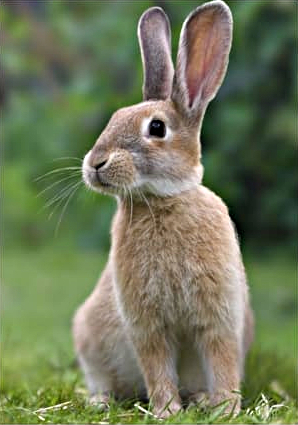
\includegraphics[height=.5\textheight]{./IMG-GIT/coelhinho.jpeg}
\end{center}
\begin{flushright}
	
\includegraphics[height=20mm]{./IMG-GIT/whatsapp.png}
\end{flushright}

	\vfill	
	\columnbreak

\begin{center}
	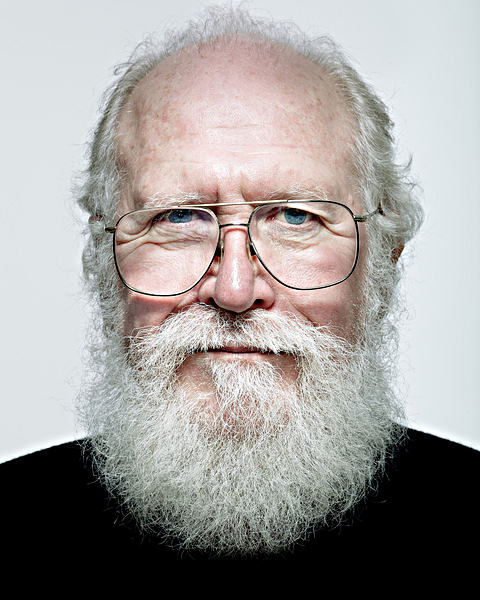
\includegraphics[height=.5\textheight]{./IMG-GIT/maddog.jpg}
\end{center}
\begin{flushright}
	
\includegraphics[height=20mm]{./IMG-GIT/whatsapp.png}
\end{flushright}
\end{multicols}	

\vfill
\pagebreak

    \ThisCenterWallPaper{1}{./IMG-GIT/ANDROMEDA.jpg}
    
\begin{multicols}{2}    
\begin{center}
	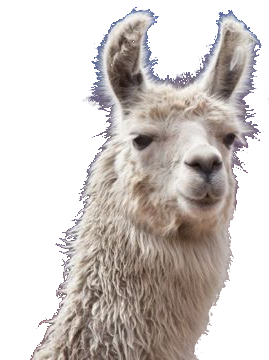
\includegraphics[height=1.15\textheight]{./IMG-GIT/lhama.png}
	
%\vspace*{-5mm}
\vfil
\columnbreak

	\resizebox{\linewidth}{15mm}{\color{white}\textbf{Lhamento!}}

%\vspace*{-15mm}	
	{\color{white}\LARGE É assim que computadores funcionam !}
\end{center}

\begin{flushright}	
	{\color{white}
		\Large
		Deseja reiniciar o Universo?
		
		
\includegraphics[width=.6\linewidth]{./IMG-GIT/yes-no.png}		
	}
\end{flushright}
\vfill
\end{multicols}


\pagebreak

 \ThisCenterWallPaper{1.05}{./IMG-GIT/spacex.jpg}

{\LARGE \color{white}Aproveite a viagem!}
	
	\vfill
	\pagebreak	
	
	\ThisCenterWallPaper{1.05}{./IMG-GIT/spacex.jpg}
	
	{\LARGE \color{white}Não esqueca sua toalha!}
		
\vfill
\pagebreak

\ThisCenterWallPaper{1}{./IMG-GIT/PALESTRANTES/flisol-latino.jpg}

{\huge Não entre em pânico!}

\vfill
\pagebreak
%\begin{multicols}{3}
%	
%	\begin{center}
%		
\includegraphics[width=\linewidth]{./IMG-GIT/PALESTRANTES/julio.jpg}
%
%	
\includegraphics[width=\linewidth]{./IMG-GIT/PALESTRANTES/junit.jpg}
%
%	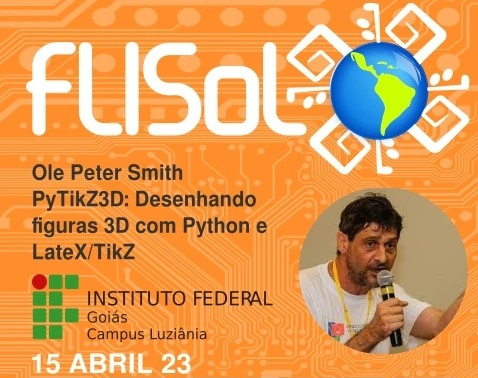
\includegraphics[width=\linewidth]{./IMG-GIT/PALESTRANTES/ole.jpg}
%
%	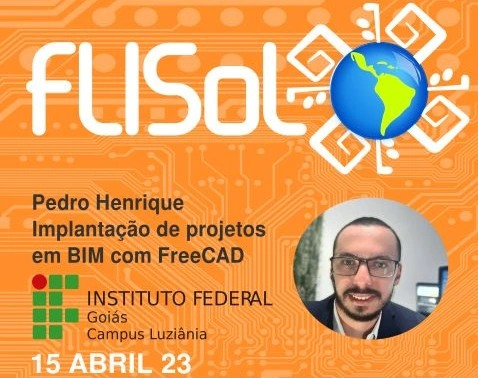
\includegraphics[width=\linewidth]{./IMG-GIT/PALESTRANTES/pedrohenriquefreecad.jpg}
%	
%	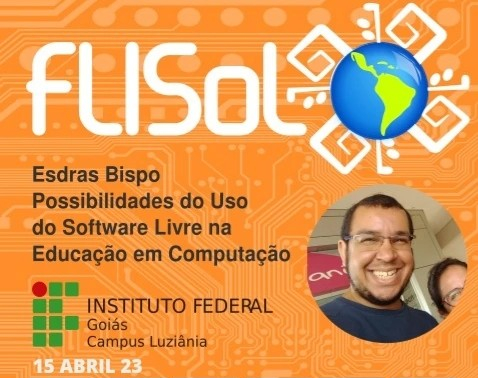
\includegraphics[width=\linewidth]{./IMG-GIT/PALESTRANTES/bispo.jpg}
%	
%	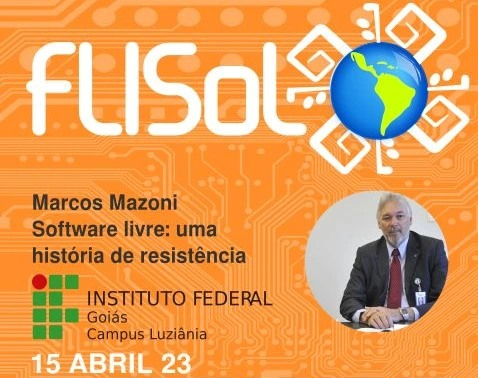
\includegraphics[width=\linewidth]{./IMG-GIT/PALESTRANTES/mazoni.jpg}
%
%\end{center}
%
%\end{multicols}

\vfill
\pagebreak

%\ThisCenterWallPaper{1}{./IMG-GIT//PALESTRANTES/aravecchia.jpg}
%
%\vfill
%\pagebreak

\ThisCenterWallPaper{1}{./IMG-GIT/SVG/DIAGRAMAS10.png}

\vspace*{.75\textheight}
{\Huge Efestus}
 \vfill
\pagebreak


%\ThisCenterWallPaper{1}{./IMG-GIT/marvin.jpg}
%
%\vspace*{2mm}
%\begin{minipage}{\linewidth}
%	\begin{minipage}[c]{0.5\linewidth}
%		
%\begin{center}
%		
\includegraphics[width=\linewidth]{./IMG-GIT/CAPA.png}
%		
%		{\LARGE 15 de abril}
%		
%%				
\includegraphics[width=.5\linewidth]{./IMG-GIT/flisol-logo.jpg}
%				
%			\resizebox{.7\linewidth}{8mm}{\color{black}sugep.ifg.edu.br}
%\end{center}
%	\end{minipage}
%	\begin{minipage}[t]{0.3\linewidth}
%%		Conteúdo da segunda minipage
%	\end{minipage}
%\end{minipage}
% 
\vfill
\pagebreak

\ThisCenterWallPaper{1}{./IMG-GIT/dontpanic.jpg}

	\Large
	
\begin{enumerate}
	\item Computadores são mais inteligentes que vogons!
	\item Armazenam e processam uma quantidade absurdamente maior de \nobreak documentos!
	\item Sao absurdamente mais rápidos!
	\item Sao honestos, confiaveis e precisos!
	\item Escrevem poesias melhores.
\end{enumerate}
	
	\vfill
	\pagebreak	
	
\begin{multicols}{2}
	\Huge Planejamento

\vfill\null
\columnbreak

			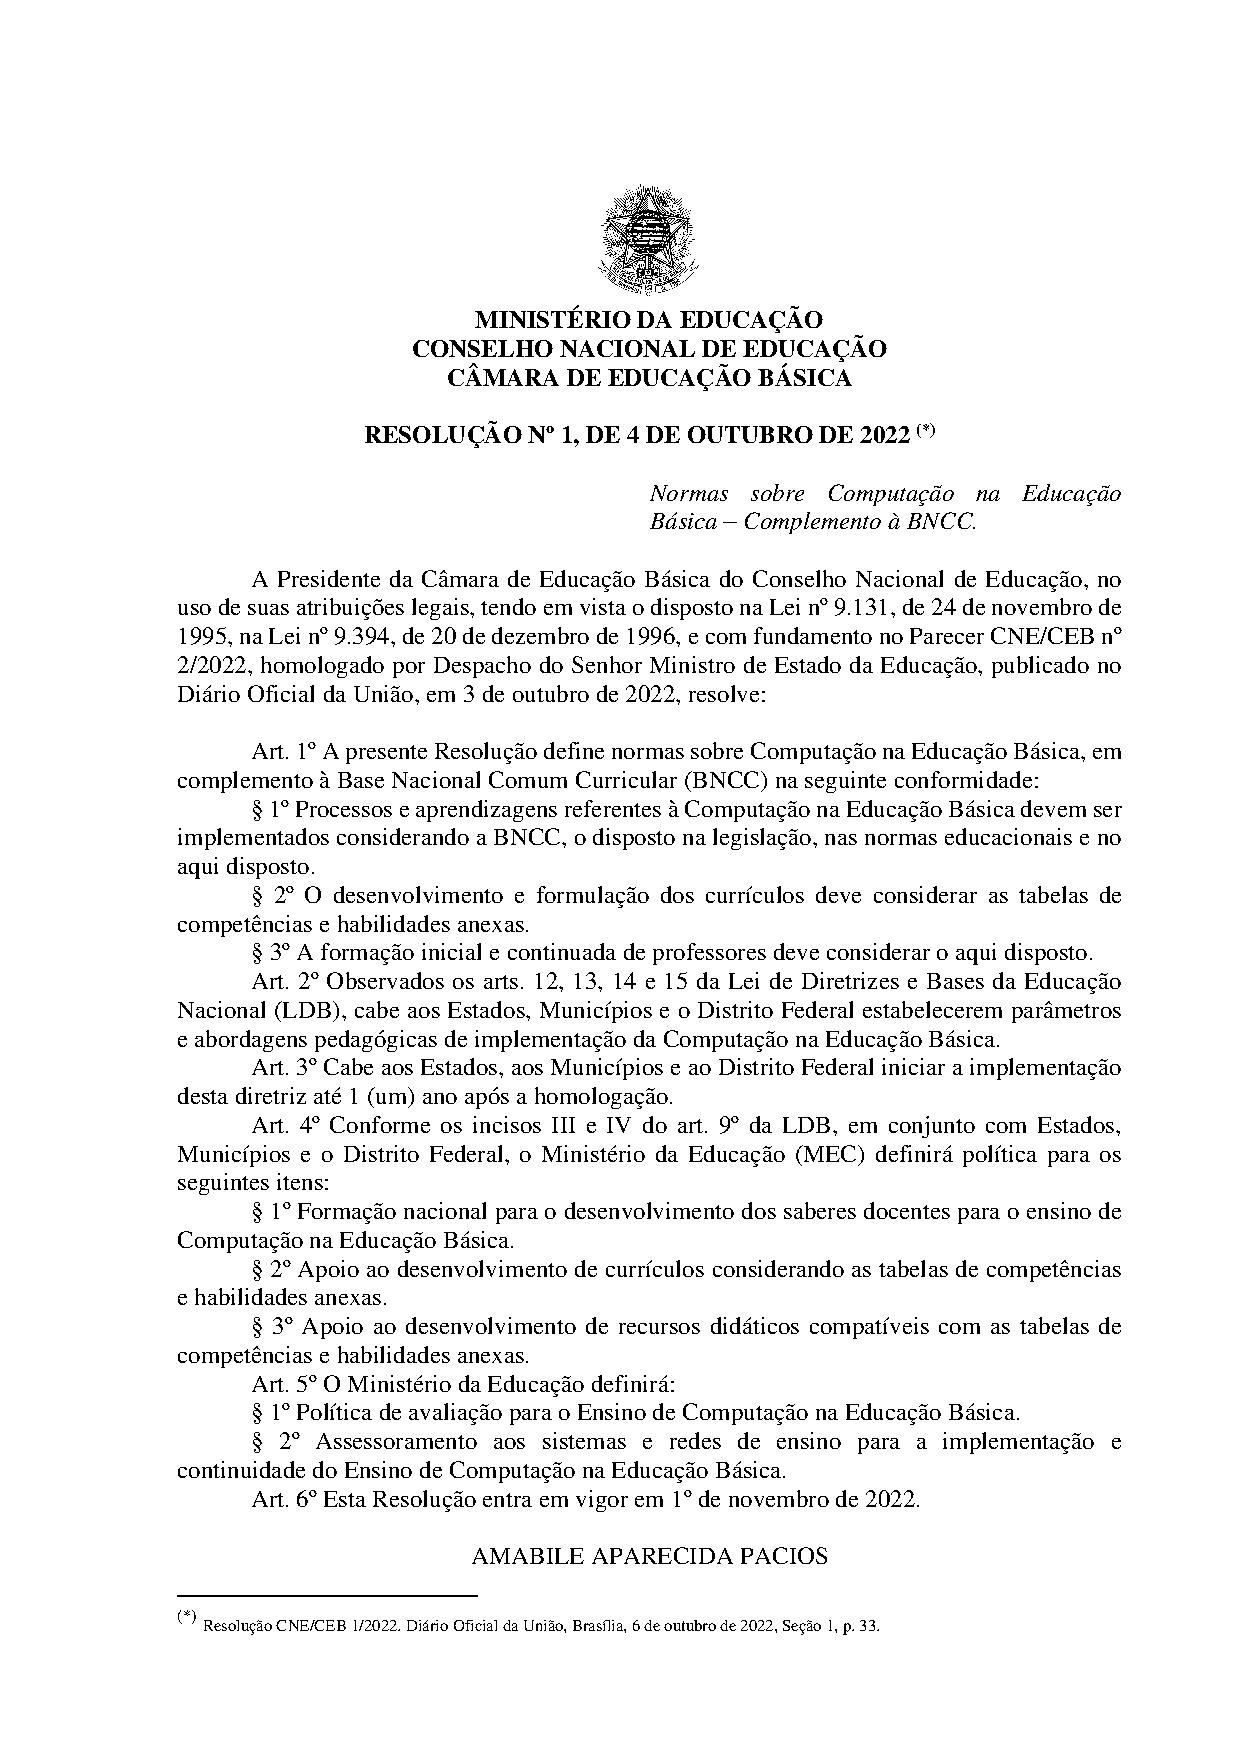
\includepdf[pages=1,height=1.5\textheight]{./PDF-GIT/RESOLUCAO-001_22.pdf}
		
\end{multicols}
		\vfill
		\pagebreak

\begin{center}
			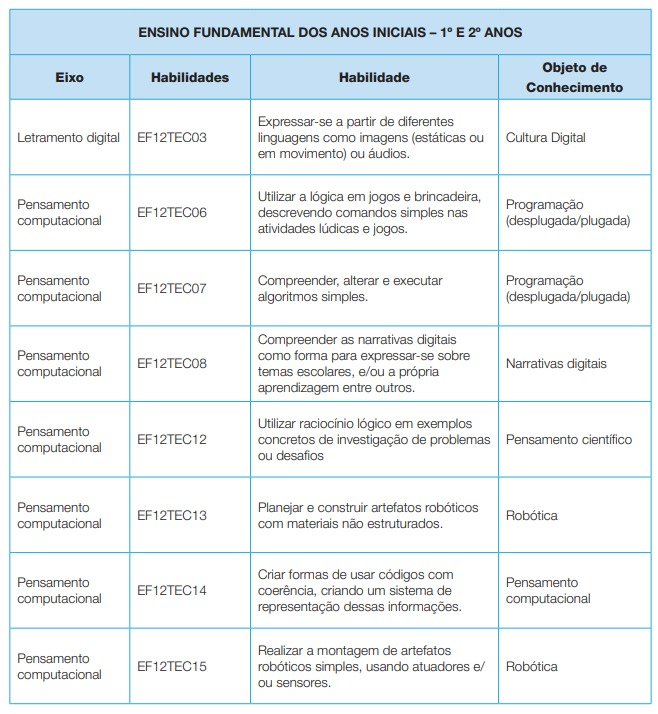
\includegraphics[height=\textheight]{./IMG-GIT/ano-1-e-2.jpeg}
\end{center}


\vfill
\pagebreak


\begin{multicols}{2}
	
\begin{itemize}	
\Large \item \textbf{Secretaria de Educação}
\item\textbf{Escola}

\large
\begin{itemize}
 	\item Direção
	\item Coordenação
	\item Conselho
\end{itemize}


\large	\item \textbf{Lista de atividades}:
\begin{itemize}
	\item EF1: 160 
	\item EF2: 128
	\item EM: 96 atividades.
\end{itemize}
\end{itemize}

\vfill\null
\columnbreak

\Large
	\begin{enumerate}
		\item Descrição sumaria da atividade
		\item Recurso computacional desejado
\begin{itemize}
		\item Texto
\begin{itemize}
	\large \item Links
	\item Aplicativos
\end{itemize}
	\item Documentos anexos:
	\begin{itemize}
		\large \item imagens
		\item videos
		\item arquivos
		\item slides
		\item musica
	\end{itemize} 
\end{itemize}
	\end{enumerate}

\vfill\null
\columnbreak

\Large
	\textbf{Laboratório de Informática}:

\begin{itemize}
	\Large
	\item \textbf{Servidor}:
	\Large 	\begin{enumerate}
\item Incorporar a Lista de Atividades ao MAIN.tex
		\item Gerar PDF com \LaTeX.
		\item Exportar de hora em hora para \textit{index.html}.
	\end{enumerate}

\vfill\null
\columnbreak

\Large
\item \textbf{Cliente}:
	\begin{enumerate}
\Large
	\item Inicialização automática do usuario aluno.
	\item Inicialização automática do navegador.
	\item Página inicial no \href{www.localhost}{\textbf{servidor}}.
	\vfill\null
	\columnbreak
		\item Diversão:
\begin{itemize}
	 \large
	 \item Scripts diversos.
	\item Acesso remoto: SSH.
	\item Horarios: \textbf{crontab}.	
	\item Liberar INDEX.html local para os alunos.
	\item Sistema de log.
	\item Gamificação.
	\item ...
\end{itemize}
\end{enumerate}
\end{itemize}
   
   \vfill\null
   \columnbreak
   
   \begin{center}
   	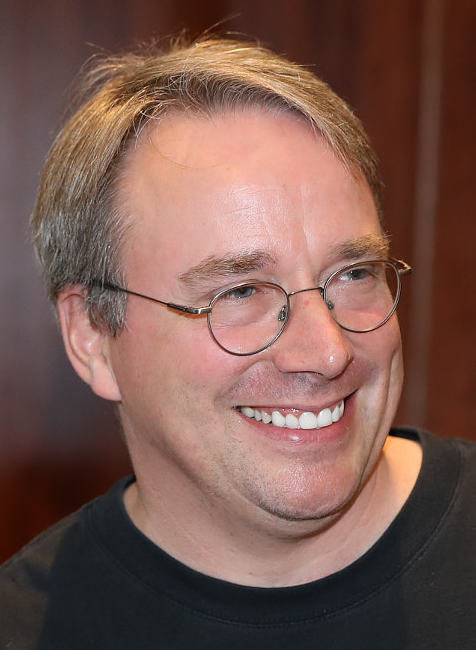
\includegraphics[height=.7\textheight]{./IMG-GIT/linus.jpeg}
   \end{center}

\LARGE \begin{enumerate}
	\item Não fale.
\item Mostre o código
\end{enumerate}
\vfill\null
\end{multicols}


\pagebreak
